\documentclass[11pt,a4paper]{scrreprt}

\usepackage[utf8]{inputenc}
\usepackage[brazil]{babel}
\usepackage[pdftex]{hyperref}
\usepackage{minted}
\usepackage{graphicx}

\title{Técnicas de Programação Avançada 2020/1}
\subtitle{Trabalho 1 -- Aclimatação com Juízes Online de Programação}
\author{Ana Carolina Cebin Pereira}
%\date{4 de Setembro de 2020}

\begin{document}

\maketitle

\chapter{Introdução}

Este trabalho tem por objetivo a resolução de problemas do sistema de juiz online de programação \href{https://open.kattis.com/}{Kattis}.

Para isso, foram resolvidos 10 problemas escolhidos entre os níveis fácil e médio e que foram submetivos e aprovados conforme os prints demonstrados, 



\chapter{Desenvolvimento}

Para o desenvolvimento das soluções foi escolhido a linguagem de Programação Python na versão 3.8.5 utilizando o Visual Code editor e executado pelo terminal


\chapter{Problemas}

\section{Basketball One-on-One}

Esta seção apresenta a solução do problema \href{https://open.kattis.com/problems/basketballoneonone}{Basketball One-on-One}.

\subsection{Características}

\begin{itemize}
    \item\textbf{TextoProblem ID: } basketballoneonone
    \item\textbf{CPU Time limit: } 1 second
    \item\textbf{Memory limit: } 1024 MB
    \item\textbf{Difficulty: }  1.4
\end{itemize}

\subsection{Código fonte}

\inputminted[linenos]{python}{src/BasketballOne-on-One.py}

\subsection{Submissão}
O programa foi submetido ao Kattis, e foi recebeu aprovação conforme demonstrado pela mensagem abaixo.

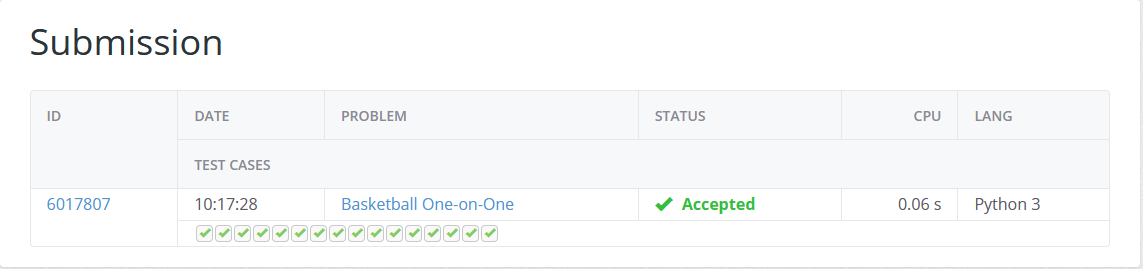
\includegraphics[scale=0.47]{img/BasketballOne-on-One.png}

\section{A Real Challenge}

Esta seção apresenta a solução do problema \href{https://open.kattis.com/problems/areal}{A Real Challenge}.

\subsection{Características}

\begin{itemize}
    \item\textbf{TextoProblem ID: } areal
    \item\textbf{CPU Time limit: } 1 second
    \item\textbf{Memory limit: } 1024 MB
    \item\textbf{Difficulty: }  1.5
\end{itemize}

\subsection{Código fonte}

\inputminted[linenos]{python}{src/ARealChallenge.py}

\subsection{Submissão}
O programa foi submetido ao Kattis, e foi recebeu aprovação conforme demonstrado pela mensagem abaixo.

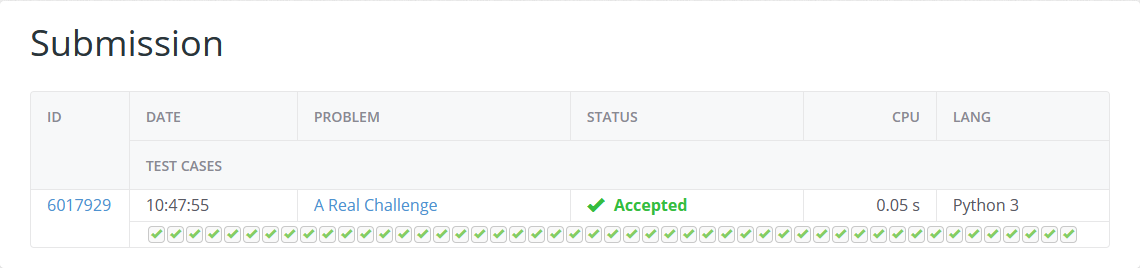
\includegraphics[scale=0.47]{img/ARealChallenge.png}

\section{Odd Man Out}

Esta seção apresenta a solução do problema \href{https://open.kattis.com/problems/oddmanout}{Odd Man Out}.

\subsection{Características}

\begin{itemize}
    \item\textbf{TextoProblem ID: } oddmanout
    \item\textbf{CPU Time limit: } 1 second
    \item\textbf{Memory limit: } 1024 MB
    \item\textbf{Difficulty: }  1.6
\end{itemize}

\subsection{Código fonte}

\inputminted[linenos]{python}{src/OddManOut.py}

\subsection{Submissão}
O programa foi submetido ao Kattis, e foi recebeu aprovação conforme demonstrado pela mensagem abaixo.

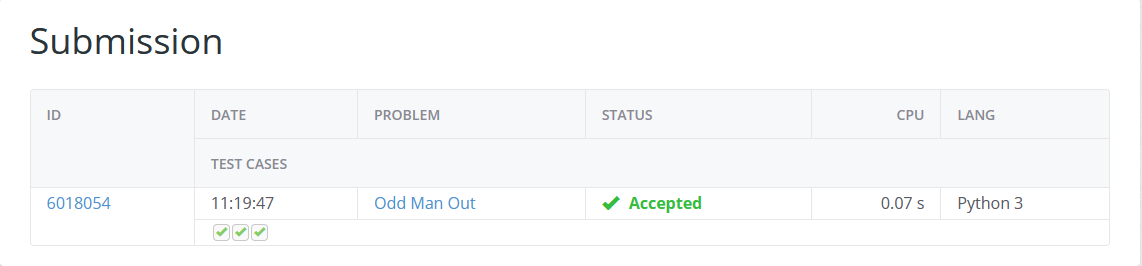
\includegraphics[scale=0.47]{img/OddManOut.png}

\section{ABC}

Esta seção apresenta a solução do problema \href{https://open.kattis.com/problems/abc}{ABC}.

\subsection{Características}

\begin{itemize}
    \item\textbf{TextoProblem ID: } abc
    \item\textbf{CPU Time limit: } 1 second
    \item\textbf{Memory limit: } 1024 MB
    \item\textbf{Difficulty: }  1.7
\end{itemize}

\subsection{Código fonte}

\inputminted[linenos]{python}{src/ABC.py}

\subsection{Submissão}
O programa foi submetido ao Kattis, e foi recebeu aprovação conforme demonstrado pela mensagem abaixo.

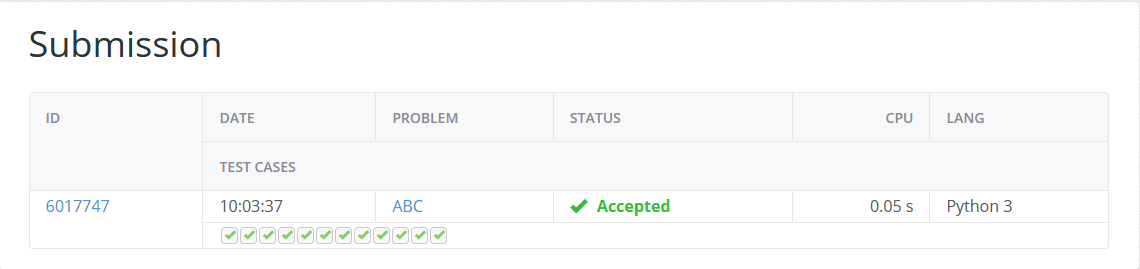
\includegraphics[scale=0.47]{img/ABC.png}

\section{Statistics}

Esta seção apresenta a solução do problema \href{https://open.kattis.com/problems/statistics}{Statistics}.

\subsection{Características}

\begin{itemize}
    \item\textbf{TextoProblem ID: } statistics
    \item\textbf{CPU Time limit: } 1 second
    \item\textbf{Memory limit: } 1024 MB
    \item\textbf{Difficulty: }  1.8
\end{itemize}

\subsection{Código fonte}

\inputminted[linenos]{python}{src/Statistics.py}

\subsection{Submissão}
O programa foi submetido ao Kattis, e foi recebeu aprovação conforme demonstrado pela mensagem abaixo.

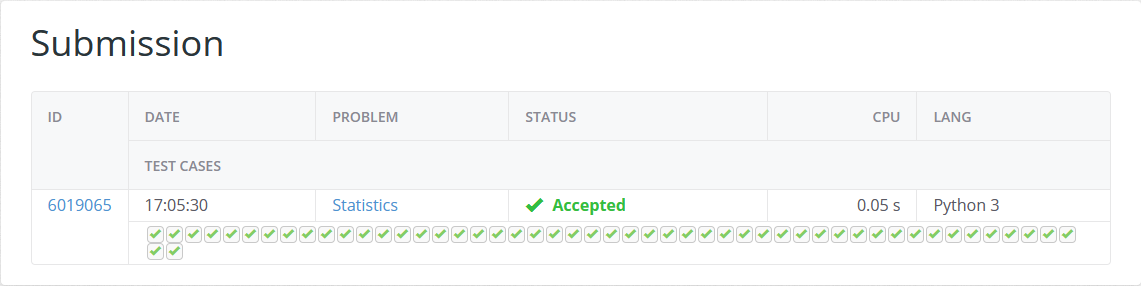
\includegraphics[scale=0.47]{img/statistics.png}

\section{Vauvau}

Esta seção apresenta a solução do problema \href{https://open.kattis.com/problems/vauvau}{Vauvau}.

\subsection{Características}

\begin{itemize}
    \item\textbf{TextoProblem ID: } vauvau
    \item\textbf{CPU Time limit: } 1 second
    \item\textbf{Memory limit: } 1024 MB
    \item\textbf{Difficulty: }  1.9
\end{itemize}

\subsection{Código fonte}

\inputminted[linenos]{python}{src/Vauvau.py}

\subsection{Submissão}
O programa foi submetido ao Kattis, e foi recebeu aprovação conforme demonstrado pela mensagem abaixo.

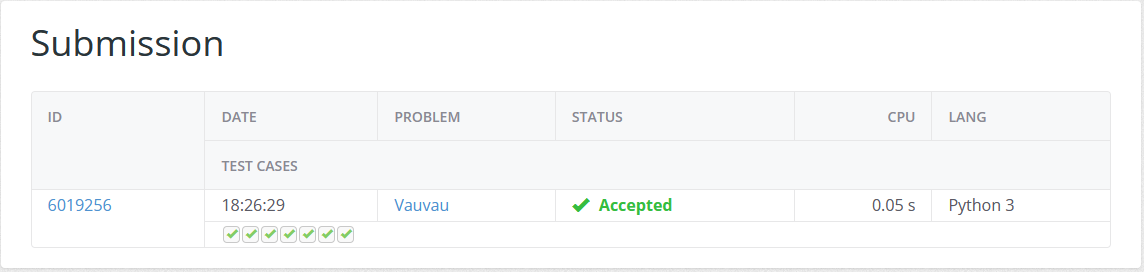
\includegraphics[scale=0.47]{img/vauvau.png}

\section{Planting Trees}

Esta seção apresenta a solução do problema \href{https://open.kattis.com/problems/plantingtrees}{Planting Trees}.

\subsection{Características}

\begin{itemize}
    \item\textbf{TextoProblem ID: } plantingtrees
    \item\textbf{CPU Time limit: } 3 second
    \item\textbf{Memory limit: } 1024 MB
    \item\textbf{Difficulty: }  2.0
\end{itemize}

\subsection{Código fonte}

\inputminted[linenos]{python}{src/PlantingTrees.py}

\subsection{Submissão}
O programa foi submetido ao Kattis, e foi recebeu aprovação conforme demonstrado pela mensagem abaixo.

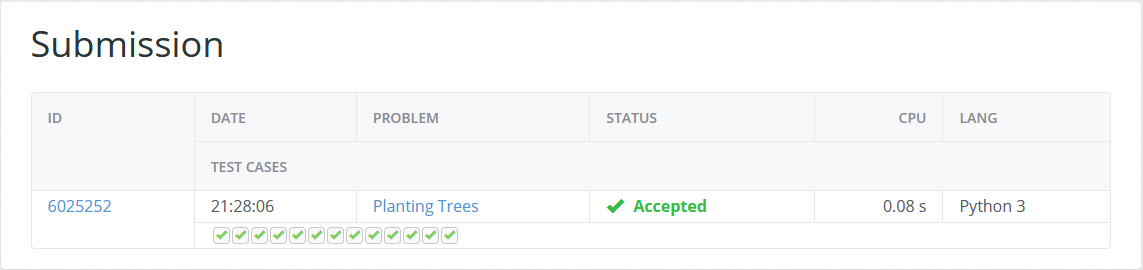
\includegraphics[scale=0.47]{img/PlantingTrees.png}


\section{Sort of Sorting}

Esta seção apresenta a solução do problema \href{https://open.kattis.com/problems/sortofsorting}{Sort of Sorting}.

\subsection{Características}

\begin{itemize}
    \item\textbf{TextoProblem ID: } sortofsorting
    \item\textbf{CPU Time limit: } 2 second
    \item\textbf{Memory limit: } 1024 MB
    \item\textbf{Difficulty: }  2.1
\end{itemize}

\subsection{Código fonte}

\inputminted[linenos]{python}{src/SortofSorting.py}

\subsection{Submissão}
O programa foi submetido ao Kattis, e foi recebeu aprovação conforme demonstrado pela mensagem abaixo.

\includegraphics[scale=0.47]{img/SortofSorting.png}

\section{A Different Problem}

Esta seção apresenta a solução do problema \href{https://open.kattis.com/problems/different}{A Different Problem}.

\subsection{Características}

\begin{itemize}
    \item\textbf{TextoProblem ID: } different
    \item\textbf{CPU Time limit: } 1 second
    \item\textbf{Memory limit: } 1024 MB
    \item\textbf{Difficulty: }  2.3
\end{itemize}

\subsection{Código fonte}

\inputminted[linenos]{python}{src/ADifferentProblem.py}

\subsection{Submissão}
O programa foi submetido ao Kattis, e foi recebeu aprovação conforme demonstrado pela mensagem abaixo.

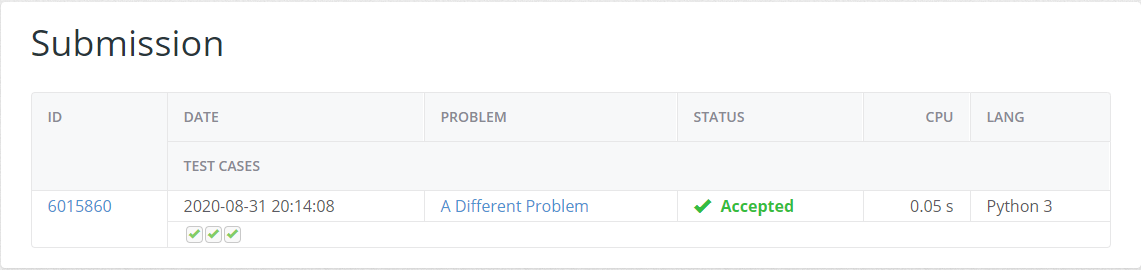
\includegraphics[scale=0.47]{img/different.png}

\section{Printing Costs}

Esta seção apresenta a solução do problema \href{https://open.kattis.com/problems/printingcosts}{Printing Costs}.

\subsection{Características}

\begin{itemize}
    \item\textbf{TextoProblem ID: } printingcosts
    \item\textbf{CPU Time limit: } 1 second
    \item\textbf{Memory limit: } 1024 MB
    \item\textbf{Difficulty: }  2.1
\end{itemize}

\subsection{Código fonte}

\inputminted[linenos]{python}{src/printingcosts.py}

\subsection{Submissão}
O programa foi submetido ao Kattis, e foi recebeu aprovação conforme demonstrado pela mensagem abaixo.

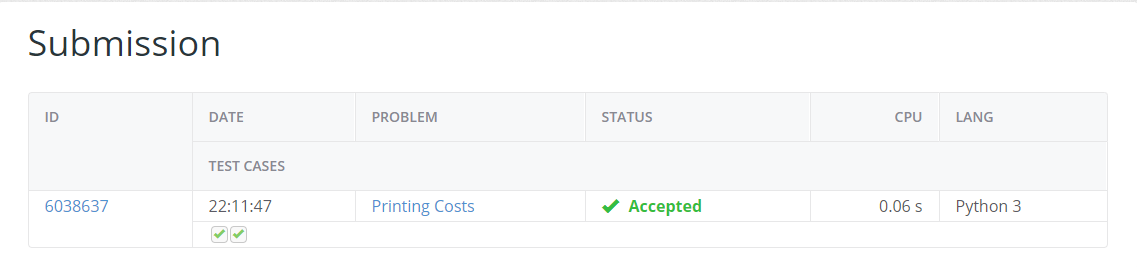
\includegraphics[scale=0.47]{img/pritingCosts.png}

\end{document}
